\documentclass[a4paper, 9pt]{article}
\usepackage{comment} 
\usepackage{graphicx}
\usepackage{fullpage}
\usepackage{hyperref}
\usepackage[italian]{babel}
\selectlanguage{italian}
\usepackage[T1]{fontenc}
\usepackage[utf8]{inputenc}
\usepackage{fontawesome}

\graphicspath{ {./images/} }

\begin{document}
\noindent
\large\textbf{Reperimento dell'Informazione} \hfill \textbf{Giovanni Candeo matr.1206150} \\
\large\textbf{Homework 1 - Report} \hfill \href{https://github.com/candeogi/HomeworkIR}{Repository GitHub \faGithub}\\
\section*{Specifiche software}
Per eseguire l'homework ho usato il seguente software:
\begin{itemize}
    \item \href{http://terrier.org/}{\textit{Terrier 4.4}} per l'indicizzazione e l'interrogazione;
    \item \href{https://trec.nist.gov/trec_eval/}{\textit{trec\_eval 9.0}} per la valutazione;
    \item Script \href{https://mathworks.com/products/matlab.html}{\textit{Matlab}} per l'analisi.
\end{itemize}

\section*{Descrizione del lavoro}
Per l'homework ho eseguito quattro run usando \textit{Terrier}, indicizzando e interrogando la collezione opportunemente seguendo le specifiche date, ovvero:
\begin{itemize}
    \item \textbf{BM25\_SL\_PS}: Stoplist, Porter stemmer, BM25  
    \item \textbf{TFIDF\_SL\_PS}: Stoplist, Porter stemmer, TF*IDF 
    \item \textbf{BM25\_PS}: No stoplist, Porter Stemmer, BM25 
    \item \textbf{TFIDF}: No stoplist, No stemmer, TF*IDF 
\end{itemize}
Per le query ho considerato entrambi i campi \textit{"title"} e \textit{"desc"} dei \textit{TREC Topic} ignorando valori con IDF troppo basso a favore di un miglioramento considerevole delle prestazioni nella run \textit{BM25\_PS}. (Vedi tabelle in basso)\\
In seguito ho valutato i risultati delle run eseguite con \textit{Terrier} usando \textit{trec\_eval}. \\ 
Per l'analisi del sistema ho usato i seguenti script e file \textit{Matlab}.
\begin{itemize}
\item \textit{textEvalToData.m} converte in due file \textit{.mat} i valori quali MAP, precision at recall base e precision at 10 dai risultati della valutazione di \textit{trec\_eval}.
\item \textit{evalData.mat} e \textit{evalAllData.mat} sono file dati risultanti da \textit{textEvalToData.m} e contengono rispettivamente i valori per ogni singolo topic e i valori calcolati per l'intera run.
\item \textit{displayTable.m} stampa una tabella per confrontare i valori tra le quattro diverse run. Utilizza il file dati \textit{evalAllData.mat}.
\item \textit{ir\_anova\_map.m, ir\_anova\_rprec.m} e \textit{ir\_anova\_p\_10.m} servono per condurre il test \textit{ANOVA 1-way} sulle varie misure. Utilizza il file dati \textit{evalData.mat}.
\end{itemize}
Preciso che ho eseguito il test \textit{ANOVA 1-way} per verificare l'equivalenza dei sistemi solo per le run che ignoravano termini con valori bassi di IDF. Boxplot e tabella con i dati del test \textit{ANOVA 1-way} sottostante si riferiscono quindi solamente a queste.
\newpage
\section*{Risultati sperimentali \& Test ANOVA}

\begin{table}[h!]
\parbox{.45\linewidth}{
\begin{tabular}{ |c|c|c|c| }
\hline
Run name& MAP & Rprec & P\_10 \\
\hline
BM25\_SL\_PS & 0.2126 & 0.2705 & 0.4840 \\
TFIDF\_SL\_PS & 0.2120 & 0.2725 & 0.4800 \\
BM25\_PS & 0.2108 & 0.2740 & 0.4740 \\
TFIDF  & 0.1875 & 0.2460 & 0.4300 \\
\hline
\end{tabular}
\caption{Risultati ottenuti ignorando termini con basso IDF}
\label{table:1}
}
\hfill
\parbox{.45\linewidth}{
\begin{tabular}{ |c|c|c|c| }
\hline
Run name & MAP & Rprec & P\_10 \\
\hline
BM25\_SL\_PS & 0.2125 & 0.2705 & 0.4820 \\
TFIDF\_SL\_PS & 0.2123 & 0.2725 & 0.4780 \\
BM25\_PS & 0.1245 & 0.1701 & 0.3020 \\
TFIDF  & 0.1876 & 0.2485 & 0.4260 \\
\hline
\end{tabular}
\caption{Risultati ottenuti non ignorando termini con basso IDF}
\label{table:1}
}
\end{table}

\begin{figure}[htp]
\centering
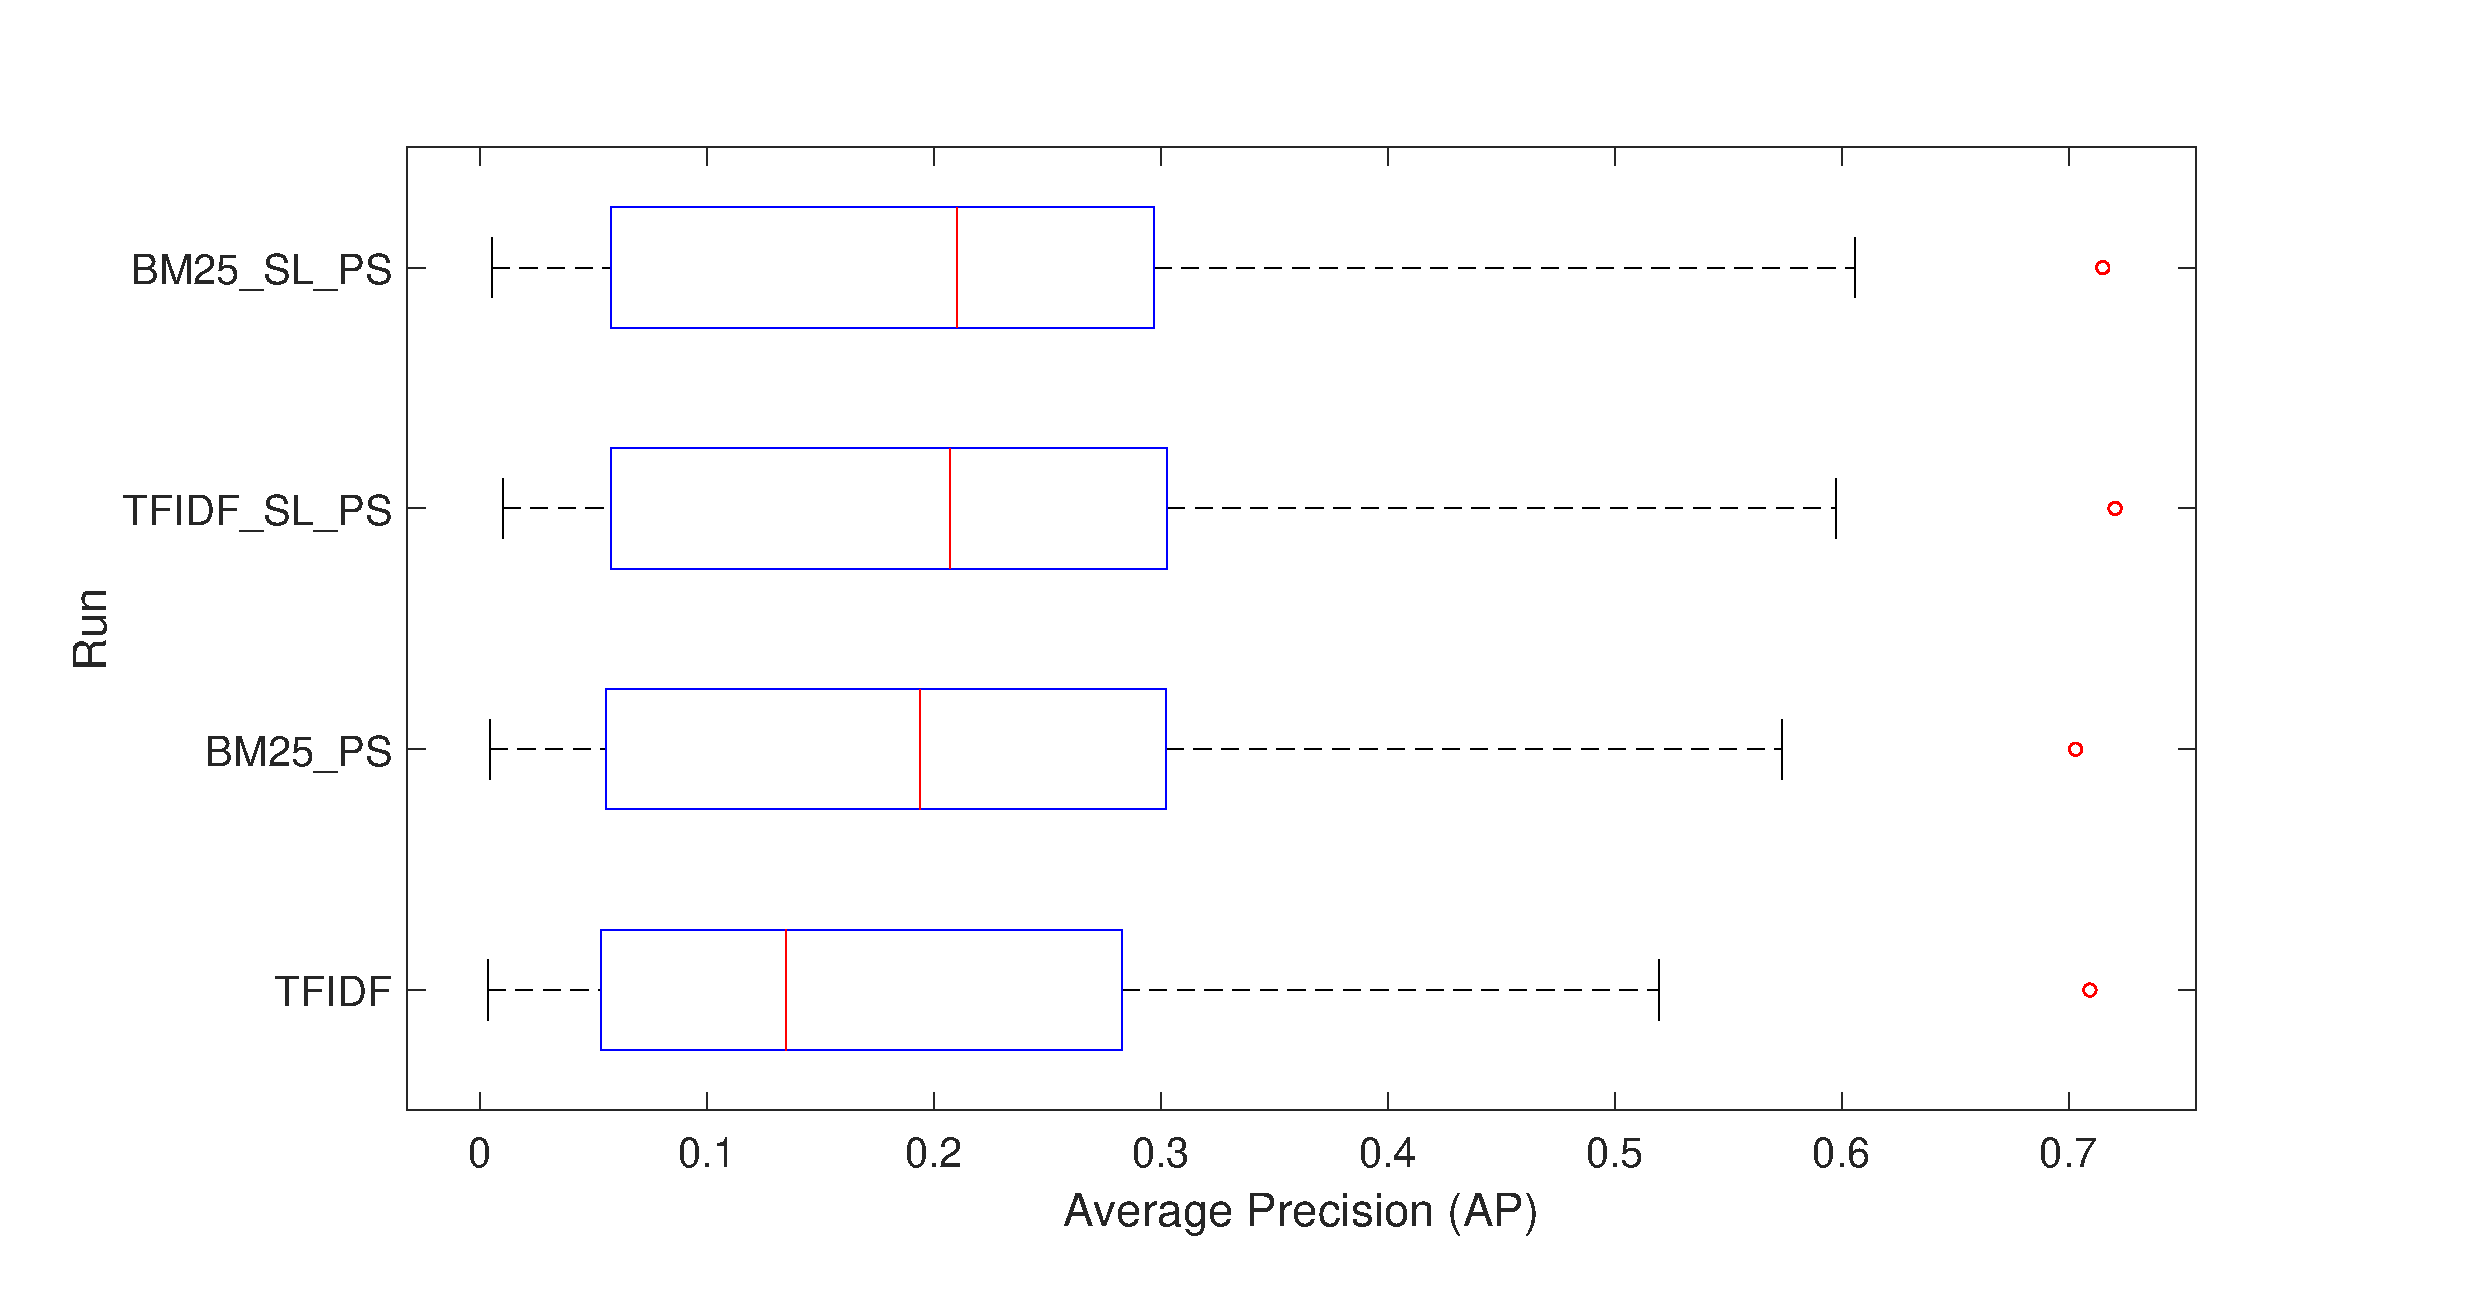
\includegraphics[width=.5\linewidth]{ap-boxplot.pdf}\hfill
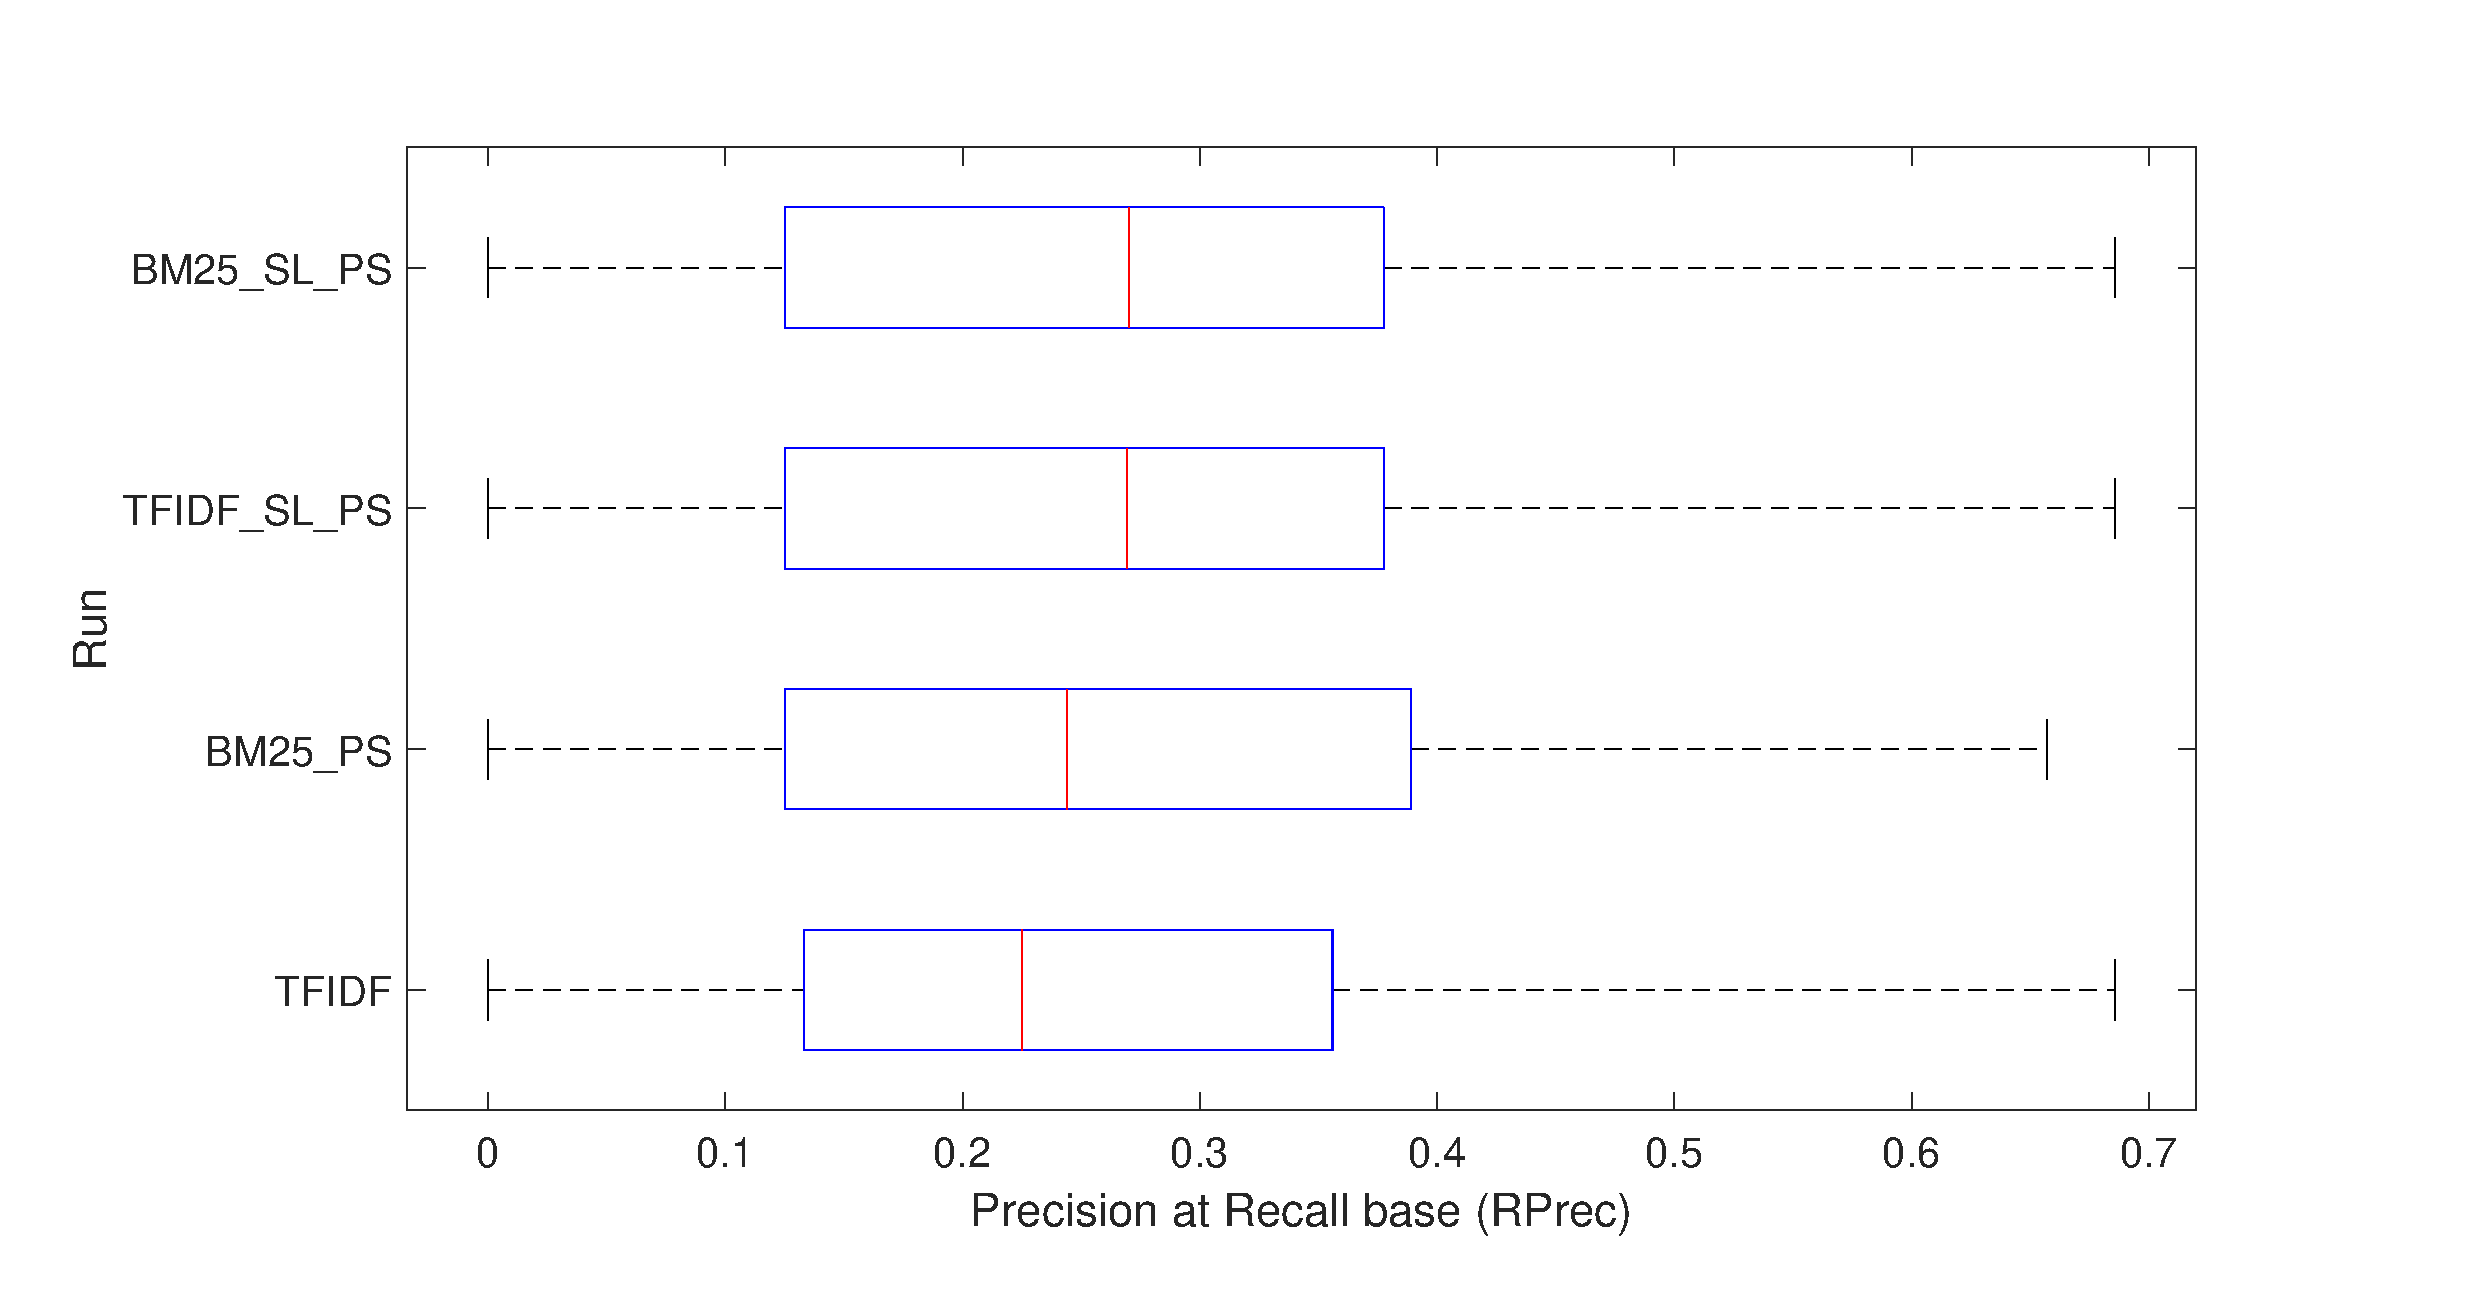
\includegraphics[width=.5\linewidth]{rprec-boxplot.pdf}
\end{figure}

% \begin{figure}[htp]
% \centering
% 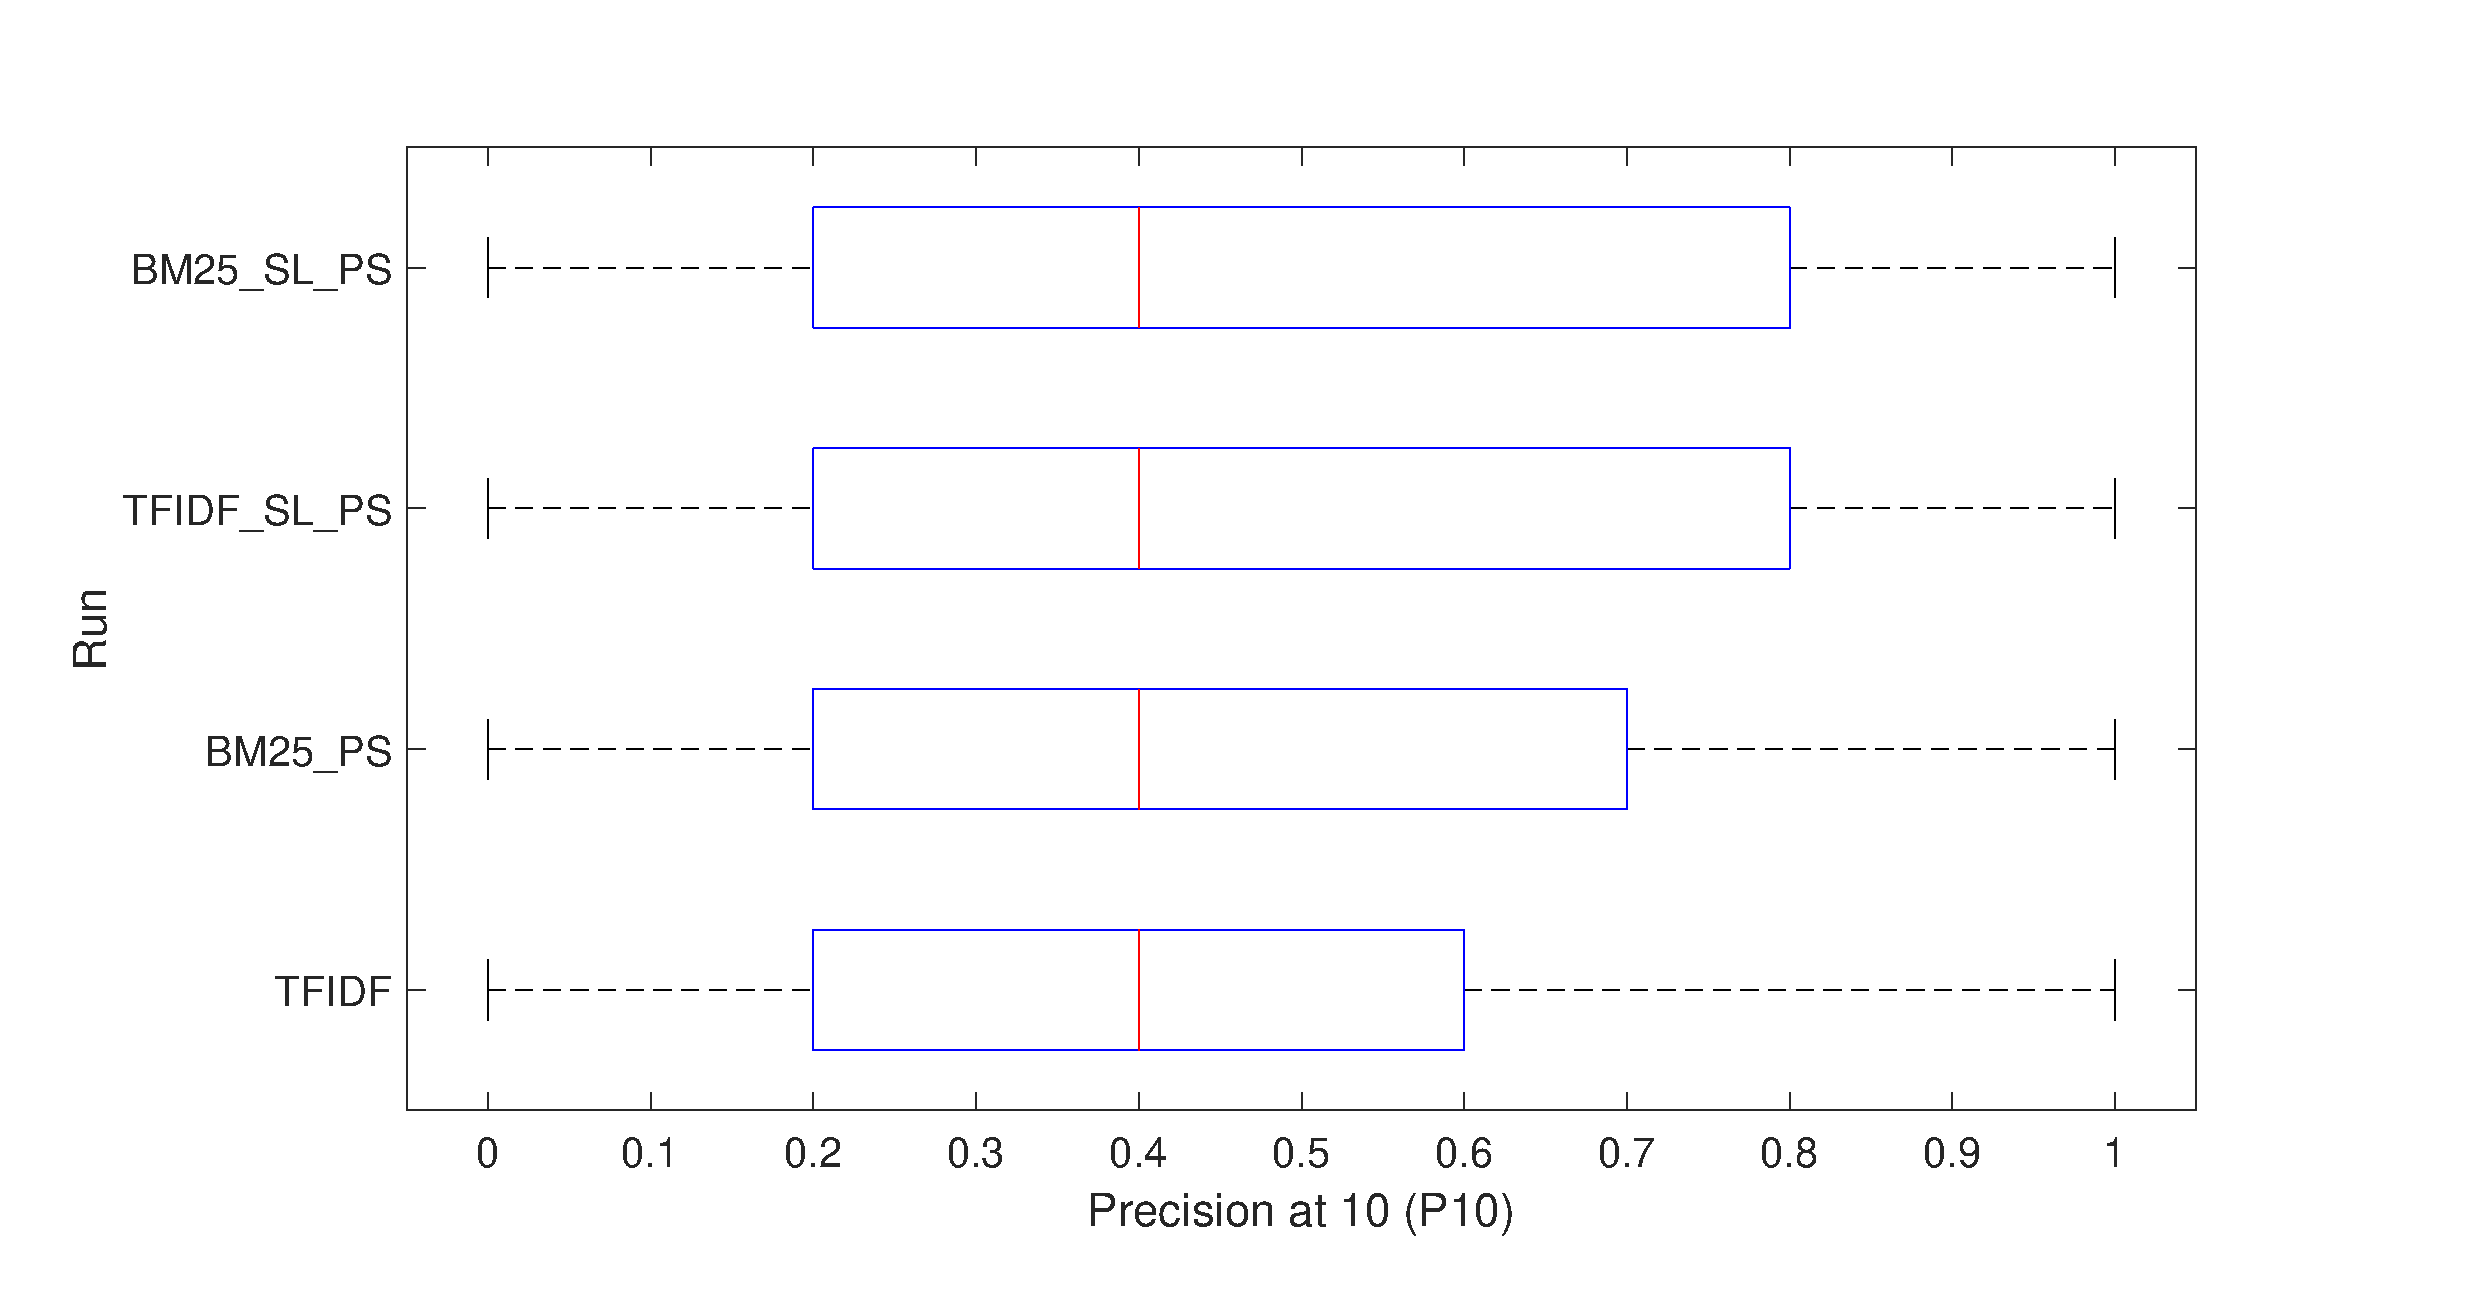
\includegraphics[width=.5\linewidth]{p10-boxplot.pdf}\hfill
% \caption{Boxplot}
% \label{fig:figure3}
% \end{figure}
\begin{figure}[htp]
\begin{minipage}[b]{0.5\linewidth}
\centering
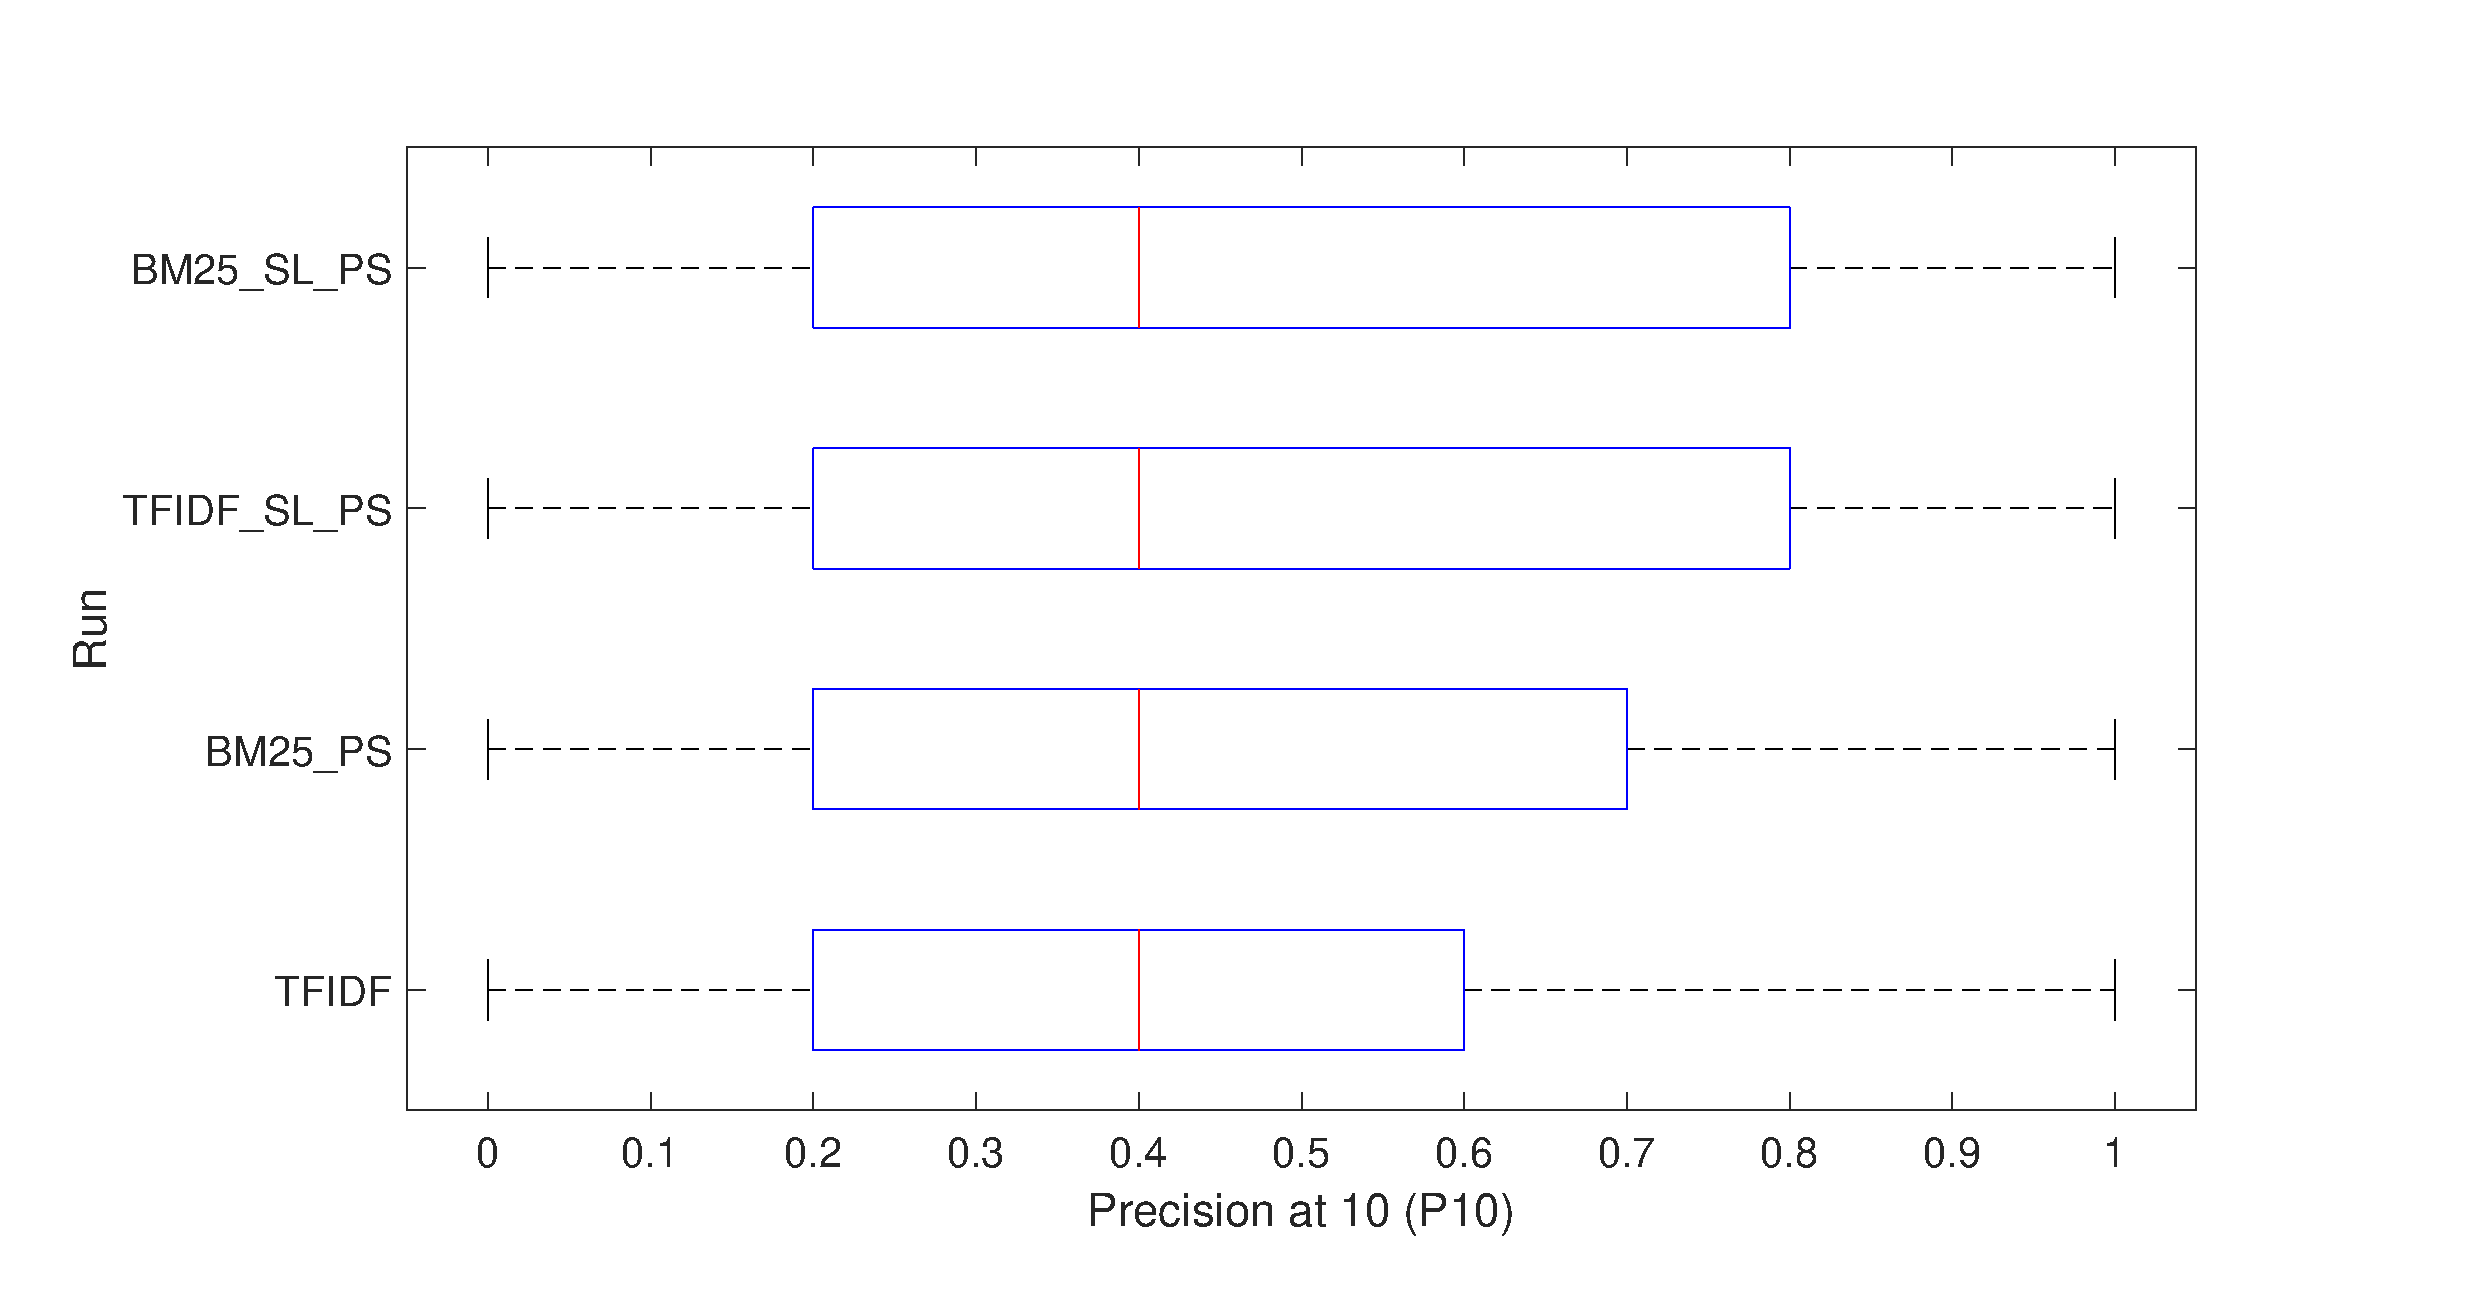
\includegraphics[width=\textwidth]{p10-boxplot.pdf}
\caption{Boxplots}
\label{fig:figure1}
\end{minipage}
\hspace{0.5cm}
\begin{minipage}[b]{0.5\linewidth}
\centering
\begin{tabular}{ |c|c|c|c| }
\hline
ANOVA & MAP & Rprec & P\_10 \\
\hline
F & 0.2698 & 0.3508 & 0.3578 \\
p value & 0.8471 & 0.7886 & 0.7836 \\
\hline
\end{tabular}
\caption{ANOVA 1-way}
\label{table:3}
\end{minipage}
\end{figure}



\subsection*{Considerazioni sui risultati: ANOVA 1-way}
\par A seguito del test \textit{ANOVA 1-way} possiamo dire che le run sono statisticamente equivalenti. 
Si nota infatti che tutti i \textit{p value} sono maggiori di 0.05, verificando quindi la \textit{null hypotesis H0}.
Eseguendo il test HSD di Tukey (script matlab per la versione interattiva presente nella repository) si può provare che tutte le run appartengono  al \textit{top-group}.
\subsection*{\textit{Considerazioni aggiuntive sui risultati: ignorare termini con basso IDF?}}
\par Ignorare o meno i termini con valore basso di IDF generalmente non cambia in modo rilevante la performance del sistema per le run di questo homework. L'unica eccezione si ha per la run \textit{BM25\_PS} dove le prestazioni per la \textit{MAP} ad esempio cambiano da 0.21 a 0.12.
Il risultato è coerente con quanto studiato nella teoria: in una run per cui in fase indicizzazione non ho filtrato \textit{stop words} sarà più probabile recuperare documenti non rilevanti che contengono quelle parole solo perchè di uso comune.
\end{document}
